\section{Progetto regolatore}

    Per progettare il regolatore dobbiamo rispettare le specifiche:
    \begin{enumerate}
        \item Errore a regime nullo prendendo come riferimento un gradino;
        \item $M_f \ge \ang{40}$;
        \item $S \% \le 1 \%$;
        \item $T_{a,5 \%} < 0.15s$;
        \item $d(t)$ deve essere abbattuto di almeno 45 dB nella banda $[0,0.08]$;
        \item $n(t)$ deve essere abbattuto di almeno 85 dB nella banda $[5\cdot 10^4, 7.5\cdot 10^7]$.
    \end{enumerate}
    $\\\\$
    Il regolatore $R(s)$ sarà formato da un regolatore statico $R_s(s)$ ed uno dinamico $R_d(s)$.\\\\
    Iniziamo a progettare il regolatore statico.\\
    Sapendo che l'errore a regime deve essere nullo se consideriamo come riferimento $W=\frac{1}{s}$
    possiamo dire che:
    \begin{equation*}
        R_s(s)=\frac{\mu_s}{s^k}
    \end{equation*}
    Da ciò sappiamo che la nostra $L(s)=R(s)G(s)$ deve avere un polo nell'origine. 
    Affinché ciò avvenga, essendo $G(s)$ priva di poli nell'origine, $R(s)$ dovrà averne uno, per 
    questo:
    \begin{equation*}
        R_s(s)=\frac{\mu_s}{s}
    \end{equation*}
    $\\$
    Prima di progettare il regolatore dinamico osserviamo più attentamente le specifiche da rispettare.
    \\\\
    Il vincolo sulla sovraelongazione si traduce in un vincolo sul margine di fase:
    \begin{equation*}
        M_f \ge \xi^* \cdot 100
    \end{equation*}
    Dove $\xi^*$ rappresenta il valore per cui viene rispettato il vincolo sulla sovraelongazione.
    Da ciò otteniamo che:
    \begin{equation*}
        \xi^* \ge \sqrt{\dfrac{\log (S^*\%)^2 }{\pi^2 + log (S^*\%)^2}} \simeq  0.826
    \end{equation*}
    con $S^*\%=1\%$\\\\
    Conseguenza di questo vincolo è che:
    \begin{equation*}
        M_f \ge \ang{82.6}
    \end{equation*}
    Questo vincolo risulta essere più stringente di quello del punto 2, per cui ci possiamo basare su 
    questo.
    $\\\\$
    La specifica sul tempo di assestamento si traduce in un vincolo su $\omega_{c_{min}}$.\\\\
    Usando l'approssimazione a poli dominanti di $F(s)$, ovvero supponendo $\omega_n \approx  \omega_c$
    e $ \xi=\xi^* $, per avere $T_{a,5 \%} < 0.15s$ deve valere 
    $\xi \cdot \omega_n \ge \frac{3}{0.15}$  , dunque:
    \begin{equation*}
        M_f \cdot \omega_c \ge \frac{3 \cdot 100}{0.15} \Rightarrow \omega_c \ge \frac{300}{0.15 \cdot 82.6}= 24 \textrm{ rad/s}
    \end{equation*}
    $\\\\$
    Per rispettare il vincolo sul rumore di uscita, studiamo il contibuto di $d(t)$ sull'uscita, ovvero:
    \begin{equation*}
        Y_d(s)=S(s)D(s)
    \end{equation*}
    Per soddisfare il vincolo vogliamo che:
    \begin{equation*}
        \lvert S(j\omega) \lvert_{dB} \le -45 \textrm{ dB} \qquad in \qquad [0,0.08]
    \end{equation*}
    In questa banda inoltre $ \lvert S(j\omega) \lvert_{dB} \approx -\lvert L(j\omega) \lvert_{dB} $, per cui il 
    vincolo diventa:
    \begin{equation*}
        \lvert L(j\omega) \lvert_{dB} \ge 45 \textrm{ dB } \qquad \omega \in [0,0.08]
    \end{equation*}
    $\\\\$
    Per rispettare il vincolo sul rumore di misura, studiamo il contibuto di $n(t)$ sull'uscita, ovvero:
    \begin{equation*}
        Y_n(s)=-F(s)N(s)
    \end{equation*}
    Per soddisfare il vincolo vogliamo che:
    \begin{equation*}
        \lvert F(j\omega) \lvert_{dB} \le -85 \textrm{ dB} \qquad in \qquad [5\cdot 10^4, 7.5\cdot 10^7]
    \end{equation*}
    In questa banda inoltre $ \lvert F(j\omega) \lvert_{dB} \approx \lvert L(j\omega) \lvert_{dB} $, per cui il 
    vincolo diventa:
    \begin{equation*}
        \lvert L(j\omega) \lvert_{dB} \le -85 \textrm{ dB } \qquad \omega \in [5\cdot 10^4, 7.5\cdot 10^7]
    \end{equation*}
    \clearpage
    Tutto ciò detto finora può essere riportato nel grafico di $G_e(s)=R_s(s)G(s)$\\
    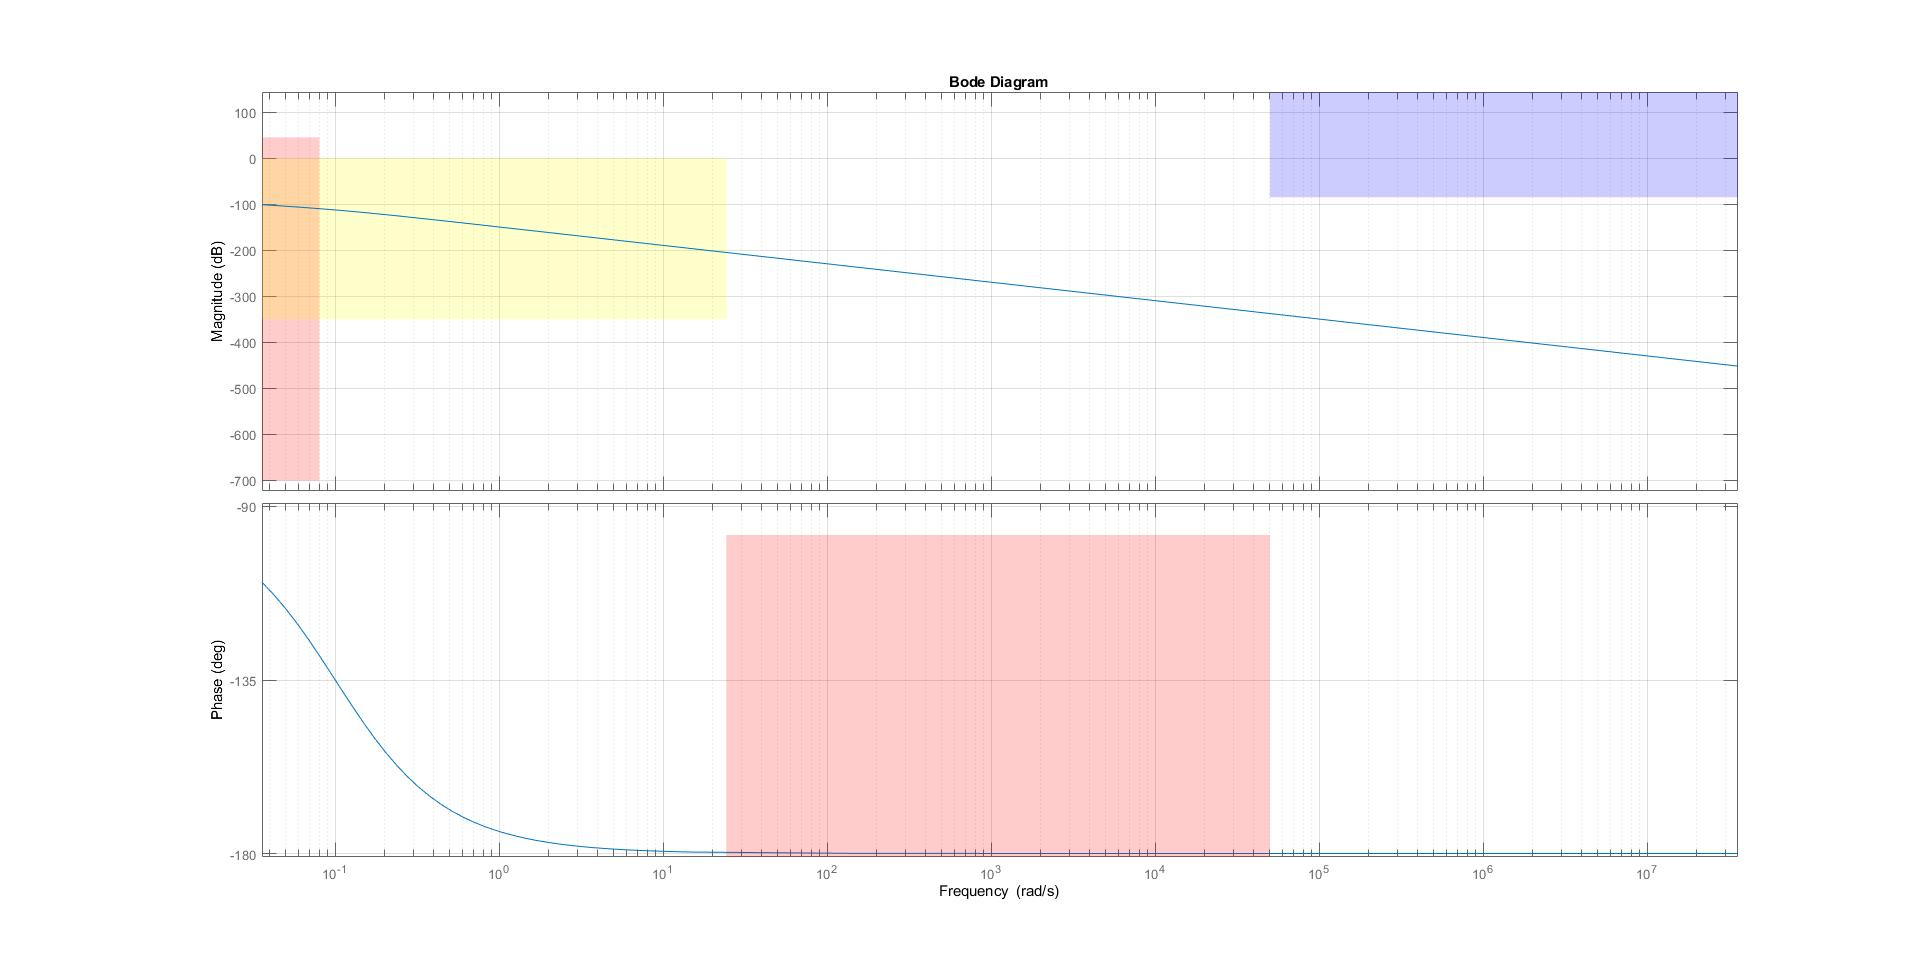
\includegraphics[scale=0.25]{./immagini/bode_ge.jpg}
    \\
    Come si può notare dalla figura, ci troviamo in uno scenario di tipo B, poiché nell'intervallo 
    in cui possiamo attraversare gli 0 dB la fase si trova sempre sotto al margine di fase imposto come limite.
    \\\\
    Per questo il nostro regolatore dinamico è una rete anticipatrice
    \begin{equation*}
        R_d(s)=\dfrac{1+\tau s}{1+\alpha \tau s}
    \end{equation*}
    Non abbiamo vincoli su $\omega_{c_{max}}$ se non quelli dovuti a $n(t)$, mentre 
    $\omega_{c_{min}}=24 \textrm{ rad/s}$ in base ai vincoli precedenti.
    \\
    Per questo abbiamo deciso di usare una pulsazione di attraversamento all'interno del 
    range definito da $\omega_{c_{min}}, \omega_{c_{max}}$ (in particolare abbiamo preso 
    $\omega_c^*=29 \textrm{ rad/s}$ ). Inoltre per essere più conservativi sul vincolo 
    relativo al margine di fase abbiamo posto $\varphi^*=\ang{89}$.
    $\\\\$
    Procediamo calcolando $M^*,\varphi^*,\tau \textrm{ e } \alpha \tau$ usando le formule di inversione:
    \begin{align*}
        &\omega_c^*=29 \textrm{ rad/s}\\
        &M_f=\ang{82.6}\\
        &M^* = 10^{-\dfrac{\lvert G_e(j \omega_c^*) \lvert_{dB}}{20}} \simeq 2.6 \cdot 10^{10}\\
        &\varphi^*= \ang{89}\\
        &\alpha \tau = \dfrac{\cos \varphi^* - \frac{1}{M^*}}{\omega_c^* \sin \varphi^*}=3.5 \cdot 10^{-4}\\
        &\tau = \dfrac{M^*-\cos \varphi^*}{\omega_c^* \sin \varphi^*}=8.8\cdot 10^8
    \end{align*}
    $\\$
    I valori calcolati di $\alpha \tau$ e $\tau$ definiscono il nostro regolatore dinamico.
    \\
    Per verificare che i vincoli siano rispettati dobbiamo osservare il comportamnto della funzione
    $L(s)$:
    \begin{equation*}
        L(s)=R_d(s)G(s)=R_d(s)R_s(s)G(s)=R(s)G(s)
    \end{equation*}
    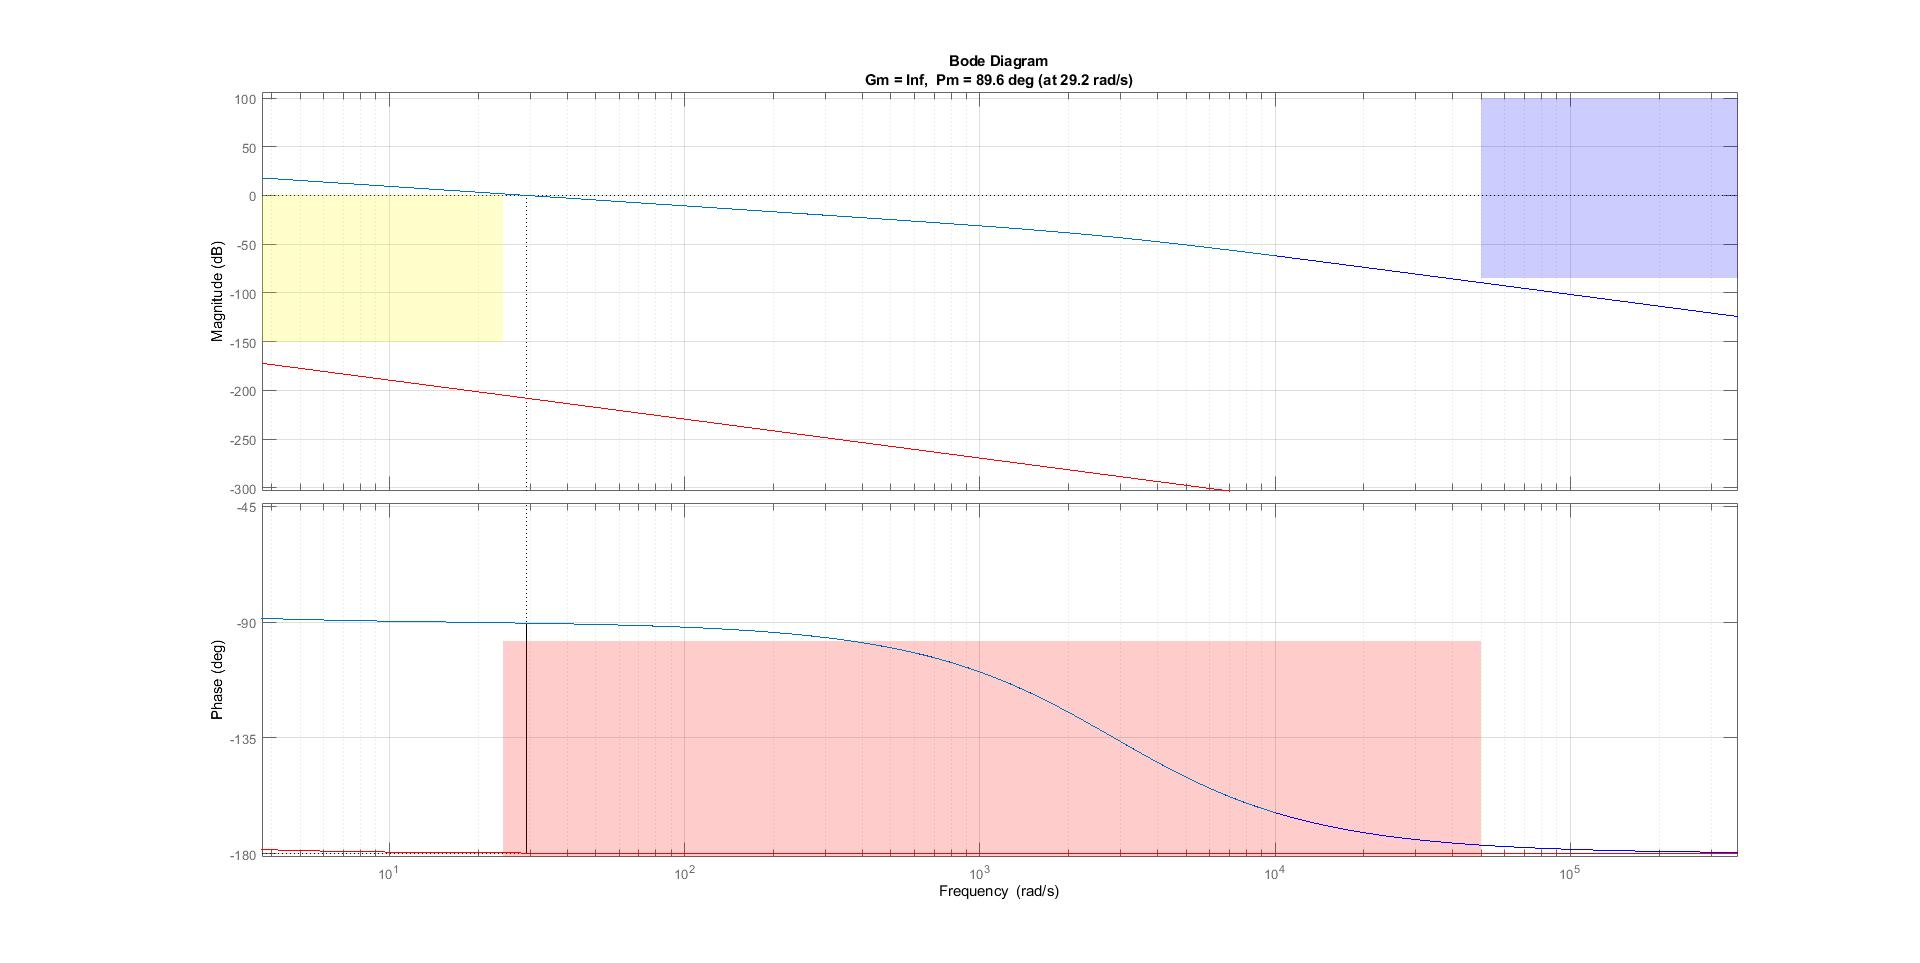
\includegraphics[scale=0.25]{./immagini/l.jpg}\\
    Nella figura si può osservare che la funzione di anello aperto rispetta i vincoli imposti.
    $\\\\$
    Infine abbiamo verificato che il sistema in anello chiuso rispetti le specifiche.
    \\
    La funzione di anello chiuso è:
    \begin{equation*}
        F(s)=\dfrac{L(s)}{1+L(s)}
    \end{equation*}
    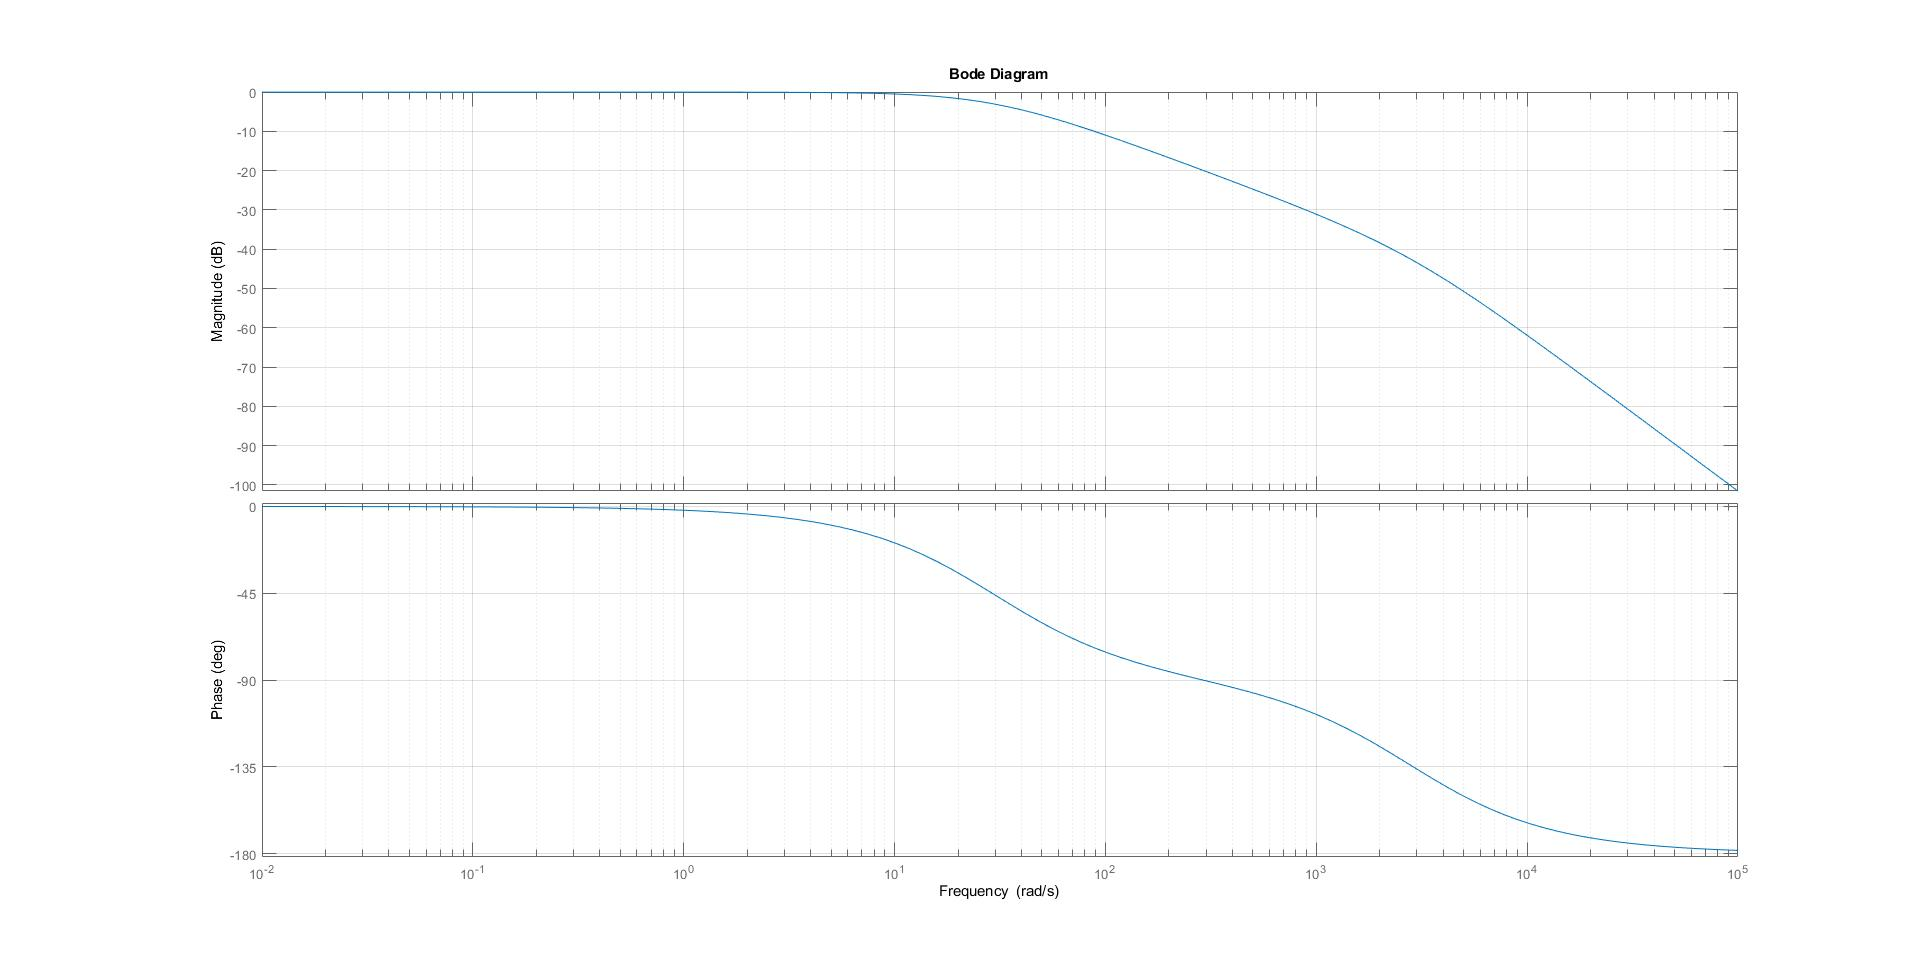
\includegraphics[scale=0.23]{./immagini/bodef.jpg}
    \clearpage
    $\\$
    Nella figura seguente si può osservare come abbiamo testato la risposta del sistema ad 
    un impulso di ampiezza unitaria, in termini di tempi di assestamento e sovraelongazione, 
    per verificare che i vincoli siano rispettati.\\
    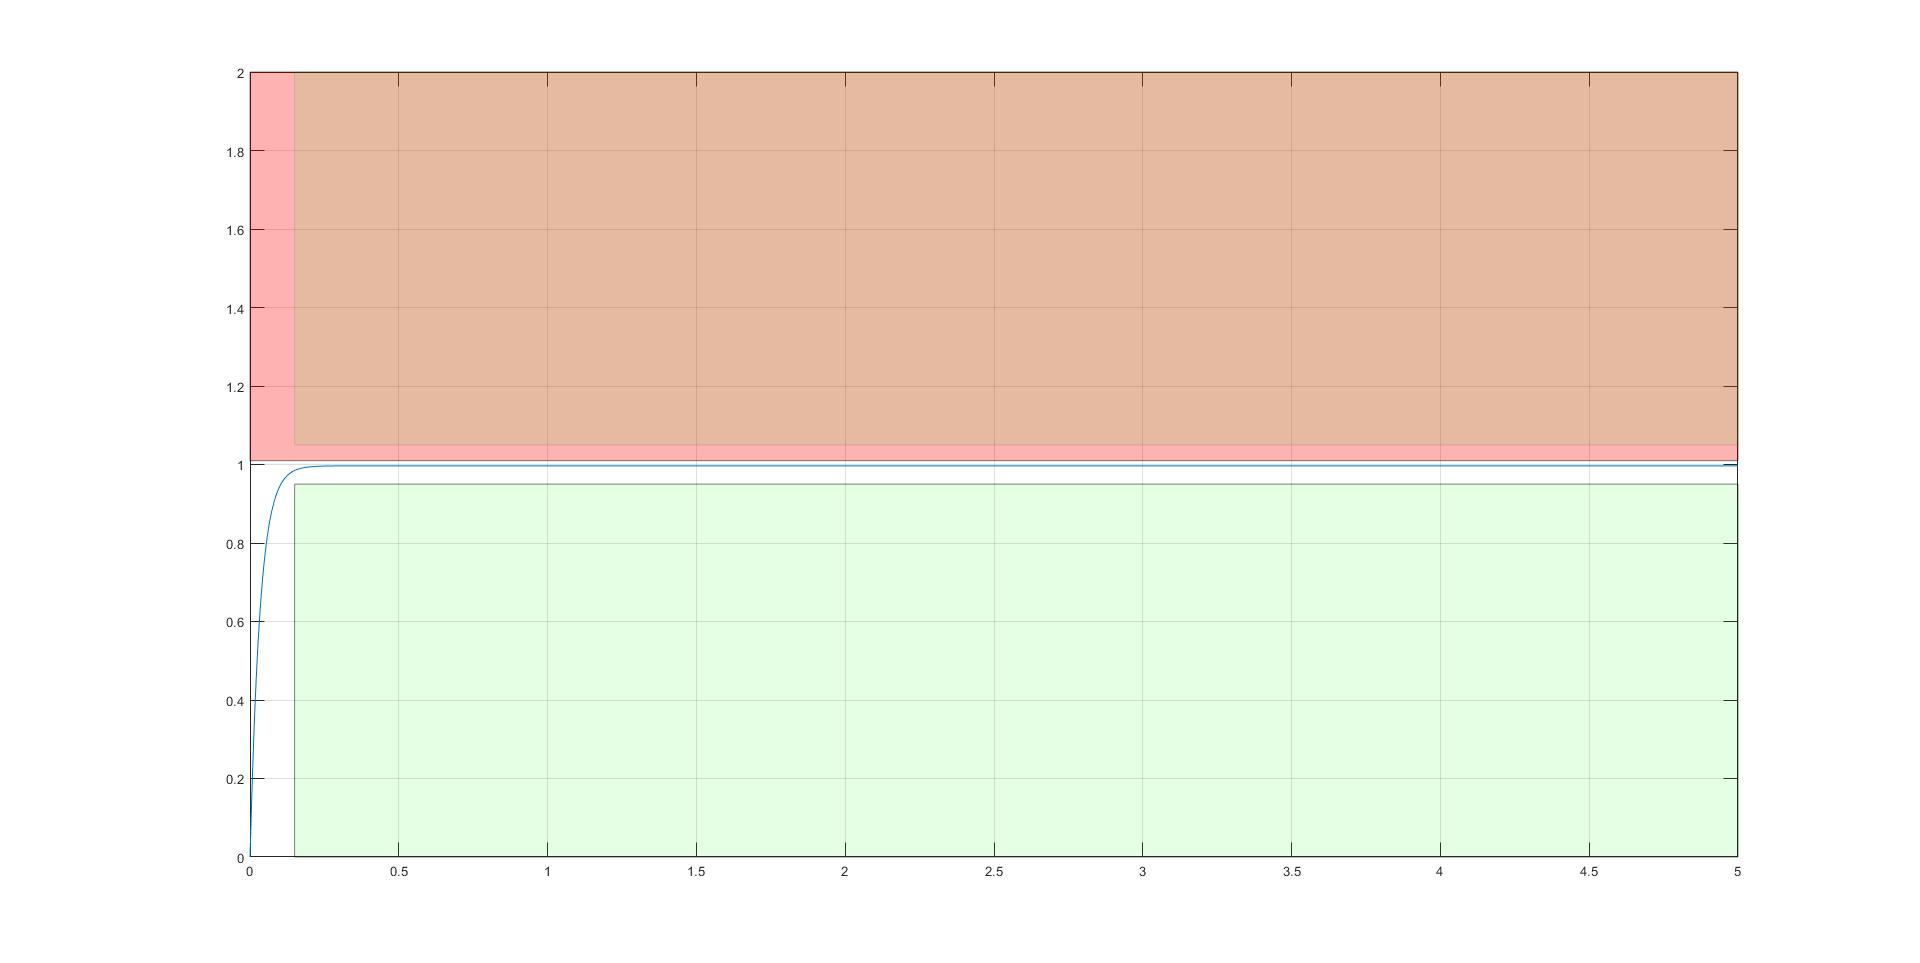
\includegraphics[scale=0.25]{./immagini/ta.jpg}
    Più nel dettaglio il patch rosso rappresenta il vincolo sulla sovraelongazione che 
    viene rispettato, come quello sul tempo di assestamento, in verde nella figura.